\chapter{Design del sistema}

\section{Introduzione}
In questo documento mostreremo delle soluzioni concrete per il modello di analisi effettuato nel documento di \docref{cha:analisi}, aggiungeremo quindi il \emph{come} al \emph{cosa}. Mostreremo quindi una specifica architetture del sistema e aggiungeremo il necessario per rendere possibile l'implementazione dei requisiti formalizzati nel documento di \docref{cha:specifica_requisiti}.

\section{Architettura del sistema}
Vengono di seguito mostrate l'architettura fisica e quella software del sistema.

\subsection{Architettura fisica}
L'architettura fisica del sistema è mostrata dalla seguente figura:
\begin{center}
   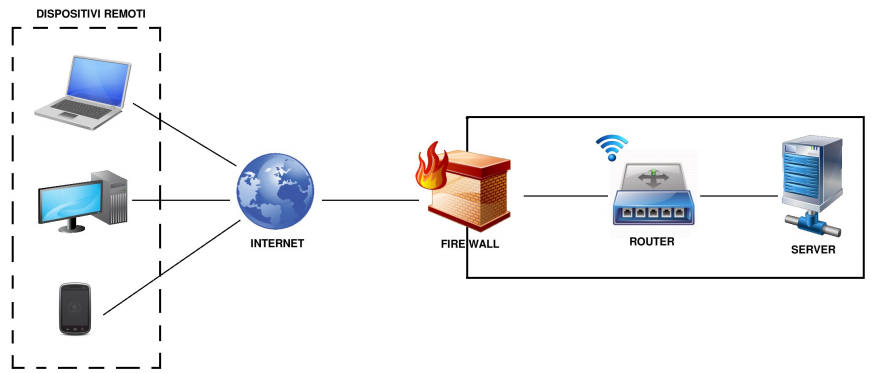
\includegraphics[width=\textwidth]{assets/architetturaFisica}
\end{center}

\subsection{Architettura software}
L'architettura software del sistema è mostrata dalla seguente figura:
\begin{center}
   \includegraphics[width=\textwidth]{assets/architetturaSoftware}
\end{center}

\section{CMS}
Per realizzare il sistema finora descritto utilizzeremo il \gls{cms} commerciale WordPress, scelto in quanto dispone di una grande quantità di plugin per soddisfare tutte le funzionalità precedentemente descritte. Questo sarà installato nel server e si occuperà della comunicazione con i fruitori del servizio e integrerà il database.

\subsection{Installazione}
Per installare WordPress sarà necessario seguire i seguenti passi:
\begin{enumerate}
	\item Scaricare e decomprimere il pacchetto di WordPress;
	\item Creare un database per WordPress sul server web, ed un utente MySQL che abbia tutti i permessi per accederci e modificarlo;
	\item Rinominare il file \texttt{wp-config-sample.php} in \texttt{wp-config.php};
	\item Aprire \texttt{wp-config.php} in un editor di testo e inserire i dettagli del database;
	\item Caricare i file di WordPress nella cartella principale del server web;
	\item Lanciare lo script di installazione di WordPress visitando la pagina \texttt{http://esempio.com/wp-admin/install.php};
\end{enumerate}

\subsection{Configurazione}
Si dovranno creare le pagine descritte in fase di analisi, abilitare l'iscrizione ed il login al sito.

\subsection{Plugin}
WordPress mette a disposizione oltre 47mila plugin, i quali estendono ed espandono le funzionalità di base presenti.
L'installazione e l'attivazione dei plugin è immediata, in quanto è possibile effettuarla direttamente tramite il pannello di controllo di WordPress.
Per implementare tutte le funzionalità precedentemente descritte sarà necessario installare ed attivare i seguenti plugin.

\subsubsection{User Role Editor}
\paragraph{Descrizione.} Con il plugin \gls{ure} è possibile cambiare le capacità di ogni ruolo. Basta spuntare le caselle di controllo delle capacità che si desidera aggiungere al ruolo selezionato. Aggiungere nuovi ruoli e personalizzarne le capacità in base alle proprie esigenze. Il ruolo creato automaticamente può essere eliminato se non ci sono utenti a cui tale ruolo è assegnato. Anche il ruolo assegnato di default alla creazione di ogni nuovo utente può essere modificato. Le capacità possono essere assegnate sulla base del singolo utente. Ruoli multipli possono essere assegnati all'utente simultaneamente. È possibile aggiungere nuove funzionalità e rimuovere le funzionalità non necessarie che potrebbero essere state lasciate da un plugin disinstallato.
\paragraph{Utilizzo.} \gls{ure} potrà essere utilizzato dall'amministratore per la gestione dei ruoli, dei profili, degli account e dell'assegnamento dei privilegi in base a quali ruoli un account possiede.
\paragraph{Configurazione.} Si dovranno creare i ruoli Visitatore, Utente, Produttore, Assistente, Redattore, Moderatore e Amministratore, assegnando ad ognuno i corrispettivi privilegi.

\subsubsection{Profile Builder Pro}
\paragraph{Descrizione.} Il plugin \gls{pbp} permette di creare profili altamente personalizzabili, è possibile inoltre personalizzare il form di iscrizione, login e recupero password. 
\paragraph{Utilizzo.}  \gls{pbp} potrà essere utilizzato per creare i profili utente e produttore, e approvare le richieste di iscrizione produttore. Potrà essere utilizzato per creare i form di registrazione per utenti e produttori.
\paragraph{Configurazione.}  Si dovranno creare i profili descritti e associarli agli account in base al loro ruolo. Si dovrà impostare l'iscrizione previa approvazione per le registrazioni di produttori. Si dovranno creare due form di registrazione: uno per gli utenti e i produttori.

\subsubsection{WP User Frontend}
\paragraph{Descrizione.} Questo plugin fornisce alle persone autenticate la possibilità di creare nuovi post, di modificare i propri profili direttamente dal fronted, senza dover accedere al pannello di amministrazione.
\paragraph{Utilizzo.}  \gls{wpuf} potrà essere utilizzato dall'amministratore per fornire alle persone autenticate la possibilità di modificare i propri profili direttamente dal frontend.
\paragraph{Configurazione.} Si dovrà dare alle persone iscritte la possibilità di personalizzare il profilo in base al ruolo posseduto.

\subsubsection{WooCommerce}
\paragraph{Descrizione.} \gls{wc} è un plugin per e-commerce gratuito che ti permette di vendere in maniera ottimale qualsiasi cosa. \gls{wc} fornisce sia ai proprietari che agli sviluppatori il controllo completo del proprio shop.
\paragraph{Utilizzo.} \gls{wc} potrà essere utilizzato per gestire la vetrina e l'inserimento e la modifica di prodotti, recensioni ad essi associate, commenti a recensioni, valutazioni e giudizi.
\paragraph{Configurazione.} Si dovrà configurare \gls{wc} in modo da non permettere la vendita di prodotti, ma solo la loro esposizione.
Per permettere a più produttori di avere la propria vetrina sarà necessaria l'installazione di \gls{wcv}.

\subsubsection{WC Vendors}
\paragraph{Descrizione.} Questo plugin permette di creare il proprio marketplace e di fornire ai venditori la possibilità di vendere come su etsy, Envato, eBay, o Amazon. \gls{wcv} permette a più venditori di vendere i propri prodotti.
\paragraph{Utilizzo.} \gls{wcv} potrà essere utilizzato per gestire più vetrine contemporaneamente, permettendo ad ogni produttore di avere la propria vetrina in cui mostrare i propri prodotti.
\paragraph{Configurazione.} Non necessita di configurazione particolare.

\subsubsection{BuddyPress}
\paragraph{Descrizione.}
BuddyPress è una insieme di componenti comuni a un tipico social network, e permette di aggiungere molte funzionalità attraverso l'esteso sistema di plugin di WordPress.
BuddyPress è focalizzato sulla facilità di integrazione, facilità d'uso e estensibilità. È un software per creare social network volutamente potente anche se incredibilmente semplice, costruito dai contributori di WordPress.
Consente ai membri di registrarsi per aprire un profilo, avere conversazioni private, effettuare collegamenti, creare per interagire nei gruppi, e molto altro. 
\paragraph{Utilizzo.}
\gls{bp} potrà essere utilizzato per gestire il lato social del sistema, oltre a gestire le richieste dagli utenti ai produttori.
\paragraph{Configurazione.}
Per configurare BuddyPress e gestire il sistema di follower/followed è necessario installare il plugin \gls{bpf}

\subsubsection{BuddyPress Follow}
\paragraph{Descrizione.}
Questo plugin permette di estendere le funzionalità di \gls{bp} per implementare il sistema di follower/followed .
\paragraph{Utilizzo.} Verrà utilizzato per implementare il sistema di follower/followed.
\paragraph{Configurazione.} Non necessita di configurazione particolare.

\subsubsection{WP Support Plus Responsive Ticket System}
\paragraph{Descrizione.} Questo plugin aggiunge a WordPress le funzionalità di un sistema di ticket completo. Permette alle persone autenticate di creare ticket per segnalare problemi o per ottenere supporto. I creatori del ticket possono impostare lo stato, la priorità e la categoria del ticket.
\paragraph{Utilizzo.} Questo plugin potrà essere utilizzato dalle persone autenticate per creare ticket per ottenere supporto.
\paragraph{Configurazione.} Non necessita di configurazione particolare.

\subsubsection{WP Report Post}
\paragraph{Descrizione.} Questo plugin permette di segnalare post o pagine con contenuti inappropriati. Tutti questi report sono mostrati in una tabella nella sezione di Amministratore, permettendo così a quest'ultimo di scegliere cosa fare: modificare i contenuti, cancellare la pubblicazione di post/pagine, o semplicemente di eliminare i report. \gls{wprp} è progettato per funzionare sia in modo automatico che in modo manuale. In modo automatico, il link per segnalare potrà essere aggiunto al meta box del post. In modo manuale, si può aggiungere il link, il bottone o l'immagine dove si vuole nel template.
\paragraph{Utilizzo.} \gls{wprp} potrà essere utilizzato per inserire la possibilità di segnalare i contenuti del sistema, come schede prodotto, recensioni o commenti.
\paragraph{Configurazione.} Si dovrà configurare il link/bottone/immagine per effettuare la segnalazione su ogni contenuto segnalabile.

\subsubsection{Ninja Forms}
\paragraph{Descrizione.} Questo plugin permette la creazione di form utilizzando un seplice drag-and-drop. Per i principianti è presente un design di creazione form semplice senza la necessità di scrivere codice. Gli sviluppatori, invece, possono utilizzare opzioni built-in, filtri, e template di campi personalizzati per la creazione di form di ogni tipo e anche per la loro sottomissione.
\paragraph{Utilizzo.} \gls{nf} potrà essere utilizzato per permettere la creazione dei form necessari all'interno del sistema.
\paragraph{Configurazione.} Non necessita di configurazione particolare.

\subsubsection{Nextend Facebook Connect}
\paragraph{Descrizione.} Questo plugin permette la registrazione ed il login tramite Facebook.
\paragraph{Utilizzo.} \gls{nfc} potrà essere utilizzato per permettere ai Visitatori di creare un account di tipo Utente utilizzando la registrazione tramite Facebook. Sarà perciò possibile effettuare il login con le credenziali di Facebook.
\paragraph{Configurazione.} Si dovranno configurare il bottone per effettuare la registrazione e quello per effettuare il login tramite Facebook.

\subsubsection{WP Search}
\paragraph{Descrizione.} Questo plugin permette la personalizzazione della ricerca in diversi modi. E' possibile assegnare pesi ai diversi tipi di contenuti, cercare in base al tipo di contenuto o in base ai tag assegnati ai contenuti. Può essere esteso grazie alle molte estensioni disponibili e mette a disposizione diverse statistiche
\paragraph{Utilizzo.} \gls{wps} potrà essere utilizzato per permettere la ricerca personalizzata in base alla tipologia di contenuto: Prodotto, Notizia o Profilo
\paragraph{Configurazione.} Si dovranno configurare la ricerca personalizzata per Prodotti, Profili e Notizie. Inserire delle opzioni per selezionare quale tipo di ricerca effettuare

\subsection{Mapping classi di analisi}
In questa sezione mostreremo come questa configurazione del \gls{cms} implementa tutte le classi di analisi descritte nel documento di \docref{cha:analisi}. Va notato che non c'è una corrispondenza biunivoca fra un sottoinsieme delle classi e un sottoinsieme dei plugin, piuttosto diversi plugin possono servire a implementare una classe o, viceversa, più classi possono essere implementate da un singolo plugin.
Si noti che le scelte progettuali effettuate rendono agevole l'espansione del sistema con ulteriori funzionalità; inoltre i possibili problemi riscontrabili solo nella fase implementativa, come ad esempio la mancanza di alcune funzionalità necessarie per il corretto funzionamento del sistema, sono facilmente risolvibili semplicemente istallando ulteriori plugin. 
Nelle seguenti pagine riportiamo il mapping effettuato fra le classi di analisi e il \gls{cms} con i suoi plugin che implementano quelle classi:
\begin{itemize}
		\item \pkgCAT{pkg:Pagine}
		\begin{itemize}	
			\item \newListItem{classe:Pagina}{\formattaCLASSE}{Pagina} 
			\item \newListItem{classe:PaginaRecensione}{\formattaCLASSE}{PaginaRecensione} 
			\item \newListItem{classe:PaginaVetrina}{\formattaCLASSE}{PaginaVetrina} 
			\item \newListItem{classe:PaginaSegnalazioni}{\formattaCLASSE}{PaginaSegnalazioni} 
			\item \newListItem{classe:PaginaTicket}{\formattaCLASSE}{PaginaTicket} 
			\item \newListItem{classe:PaginaNotizie}{\formattaCLASSE}{PaginaNotizie} 
			\item \newListItem{classe:PaginaProfilo}{\formattaCLASSE}{PaginaProfilo} 
			\item \newListItem{classe:PaginaRichiesteIscrizioni}{\formattaCLASSE}{PaginaRichiesteIscrizioni} 
			\item \newListItem{classe:PaginaLogin}{\formattaCLASSE}{PaginaLogin} 
			\item \newListItem{classe:PaginaSchedaProdotto}{\formattaCLASSE}{PaginaSchedaProdotto} 			
			\item \newListItem{classe:PaginaAggiornamentiFollower}{\formattaCLASSE}{PaginaAggiornamentiFollower} 
			\item \newListItem{classe:PaginaRichiesteProdotto}{\formattaCLASSE}{PaginaRichiesteProdotto} 
			\item \newListItem{classe:PaginaIscrizione}{\formattaCLASSE}{PaginaIscrizione} 
			\item \newListItem{classe:Home}{\formattaCLASSE}{Home} 
		\end{itemize}	
		\item \pkgCAT{pkg:GestioneContenuti}
		\begin{itemize}	
			\item \newListItem{classe:GestioneSchedaProdotto}{\formattaCLASSE}{GestioneSchedaProdotto} 
			\item \newListItem{classe:GestioneNotizia}{\formattaCLASSE}{GestioneNotizia} 
			\item \newListItem{classe:GestioneRecensione}{\formattaCLASSE}{GestioneRecensione} 
		\end{itemize}	
		\item \pkgCAT{pkg:GestioneProfili}
		\begin{itemize}	
			\item \newListItem{classe:GestioneProfilo}{\formattaCLASSE}{GestioneProfilo} 
			\item \newListItem{classe:GestioneVetrina}{\formattaCLASSE}{GestioneVetrina} 
		\end{itemize}	
		\item \pkgCAT{pkg:GestioniComunicazioni}
		\begin{itemize}	
			\item \newListItem{classe:GestioneRichiesteProdotto}{\formattaCLASSE}{GestioneRichiesteProdotto} 
			\item \newListItem{classe:GestioneSegnalazioni}{\formattaCLASSE}{GestioneSegnalazioni} 
			\item \newListItem{classe:GestioneTicket}{\formattaCLASSE}{GestioneTicket} 
		\end{itemize}	
		\item \pkgCAT{pkg:GestioneSistema}
		\begin{itemize}	
			\item \newListItem{classe:GestioneAccessi}{\formattaCLASSE}{GestioneAccessi} 
			\item \newListItem{classe:GestioneIscritti}{\formattaCLASSE}{GestioneIscritti} 
			\item \newListItem{classe:Utility}{\formattaCLASSE}{Utility} 
			\item \newListItem{classe:Ricerca}{\formattaCLASSE}{Ricerca} 
		\end{itemize}	
		\item \pkgCAT{pkg:Contenuti}
		\begin{itemize}	
			\item \newListItem{classe:Contenuto}{\formattaCLASSE}{Contenuto} 
			\item \newListItem{classe:Commento}{\formattaCLASSE}{Commento} 
			\item \newListItem{classe:Recensione}{\formattaCLASSE}{Recensione} 
			\item \newListItem{classe:Giudizio}{\formattaCLASSE}{Giudizio} 
			\item \newListItem{classe:SchedaProdotto}{\formattaCLASSE}{SchedaProdotto} 
			\item \newListItem{classe:Valutazione}{\formattaCLASSE}{Valutazione} 
			\item \newListItem{classe:Notizia}{\formattaCLASSE}{Notizia} 
			\item \newListItem{classe:ConsistenzaProdotto}{\formattaCLASSE}{ConsistenzaProdotto} 
			\item \newListItem{classe:CategoriaProdotto}{\formattaCLASSE}{CategoriaProdotto} 
		\end{itemize}	
		\item \pkgCAT{pkg:Comunicazioni}
		\begin{itemize}	
			\item \newListItem{classe:Ticket}{\formattaCLASSE}{Ticket} 
			\item \newListItem{classe:RichiestaProduttore}{\formattaCLASSE}{RichiestaProduttore} 
			\item \newListItem{classe:RispostaTicket}{\formattaCLASSE}{RispostaTicket} 
			\item \newListItem{classe:RichiestaProdotto}{\formattaCLASSE}{RichiestaProdotto} 
			\item \newListItem{classe:SegnalazioneContenuto}{\formattaCLASSE}{SegnalazioneContenuto} 
		\end{itemize}	
		\item \pkgCAT{pkg:Iscrizioni}
		\begin{itemize}	
			\item \newListItem{classe:Account}{\formattaCLASSE}{Account} 
			\item \newListItem{classe:TipoAccount}{\formattaCLASSE}{TipoAccount} 
			\item \newListItem{classe:RichiestaIscrizione}{\formattaCLASSE}{RichiestaIscrizione} 
			\item \newListItem{classe:Privilegi}{\formattaCLASSE}{Privilegi} 
		\end{itemize}	
		\item \pkgCAT{pkg:Profili}
		\begin{itemize}	
			\item \newListItem{classe:Profilo}{\formattaCLASSE}{Profilo} 
			\item \newListItem{classe:ProfiloProduttore}{\formattaCLASSE}{ProfiloProduttore} 
			\item \newListItem{classe:Vetrina}{\formattaCLASSE}{Vetrina} 
		\end{itemize}	
		\item \pkgCAT{pkg:Autenticazione}
		\begin{itemize}	
			\item \newListItem{classe:AccessoIscritto}{\formattaCLASSE}{AccessoIscritto} 
			\item \newListItem{classe:AccessoOspite}{\formattaCLASSE}{AccessoOspite} 
		\end{itemize}	
		\item \pkgCAT{pkg:Utility}
		\begin{itemize}	
			\item \newListItem{classe:TipoRicerca}{\formattaCLASSE}{TipoRicerca} 
		\end{itemize}	
\end{itemize}

\classeTab{classe:Pagina}
{\acrlong{wp}}
{\acrlong{wp} gestisce senza necessità di particolari plugin la creazione di pagine semplici}

\vspaceTab

\classeTab{classe:PaginaRecensione}
{\acrlong{wp}, \acrlong{wc}}
{\acrlong{wp} gestisce la creazione delle pagine, mentre il plugin \acrlong{wc} gestisce la visualizzazione delle recensioni}

\vspaceTab

\classeTab{classe:PaginaVetrina}
{\acrlong{wp}, \acrlong{wc}, \acrlong{wcv}}
{\acrlong{wp} gestisce la creazione delle pagine, il plugin \acrlong{wc} gestisce la visualizzazione delle recensioni mentre il plugin \acrlong{wcv} permette di avere negozi multipli (una vetrina per ogni produttore presente)}

\vspaceTab

\classeTab{classe:PaginaSegnalazioni}
{\acrlong{wp}, \acrlong{wprp}}
{\acrlong{wp} gestisce la creazione delle pagine, mentre \acrlong{wprp} gestisce l'intero sistema di segnalazioni con relativa visualizzazione da parte di un moderatore delle stesse}

\vspaceTab

\classeTab{classe:PaginaTicket}
{\acrlong{wp}, \acrlong{wpsprts}}
{\acrlong{wp} gestisce la creazione delle pagine, mentre \acrlong{wpsprts} gestisce l'intero sistema di tiket con relativa visualizzazione da parte di un assistente delle stesse}

\vspaceTab

\classeTab{classe:PaginaNotizie}
{\acrlong{wp}}
{\acrlong{wp} gestisce senza necessità di particolari plugin la creazione di pagine contenenti notizie}

\vspaceTab

\classeTab{classe:PaginaProfilo}
{\aprlong{wp}, \acrlong{pbp}}
{\aprlong{wp} gestisce la creazione delle pagine profilo, \aprlong{pbp} permette agli amministratori di creare profili personalizzati in base al tipo di account}

\vspaceTab 

\classeTab{classe:PaginaRichiesteIscrizioni}
{\acrlong{wp}, \acrlong{pbp}}
{\acrlong{wp} gestisce la creazione delle pagine contenenti le richieste di iscrizione, \acrlong{pbp} permette agli assistenti di visualizzare le richieste d'iscrizione delle persone che si iscrivono tramite il form d'iscrizione produttori}

\vspaceTab

\classeTab{classe:PaginaLogin}
{\acrlong{wp}, \acrlong{nfc}}
{\acrlong{wp} gestisce la creazione della pagina di Login, \acrlong{nfc} permette l'accesso tramite Facebook}

\vspaceTab

\classeTab{classe:PaginaSchedaProdotto}
{\acrlong{wp}, \acrlong{wc}, \acrlong{wcv}, \acrlong{nf}}
{\acrlong{wp} gestisce la creazione delle pagine prodotto, \acrlong{wc} e \acrlong{wcv} permettono ai produttori di mostrare i propri prodotti, \acrlong{nf} permette di personalizzare i campi della scheda prodotto}

\vspaceTab

\classeTab{classe:PaginaAggiornamentiFollower}
{\acrlong{wp}, \acrlong{bp}, \acrlong{bpf}}
{\acrlong{wp} gestisce la creazione delle pagine in cui si possono visualizzare gli aggiornamenti delle persone che si seguono, \acrlong{bp} esteso con \acrlong{bpf} implementa le funzionalità di follower/followed}

\vspaceTab

\classeTab{classe:PaginaRichiesteProdotto}
{\acrlong{wp}, \acrlong{bp}, \acrlong{nf}}
{\acrlong{wp} gestisce la creazione delle pagine contenenti le richieste prodotto, \acrlong{bp} permette di visualizzare le richieste prodotto ricevute, \acrlong{nf} permette la gestione dei form delle richieste prodotto}

\vspaceTab

\classeTab{classe:PaginaIscrizione}
{\acrlong{wp}, \acrlong{pbp}, \acrlong{nfc}}
{\acrlong{wp} gestisce la creazione delle pagine di iscrizione, \acrlong{pbp} permette di creare form di iscrizione multipli, quindi un form per l'iscrizione di account che otterrano ruolo utente e uno per quelli che otterrano ruolo produttore, \acrlong{nfc} permette di effettuare l'iscrizione direttamente con le credenziali di Facebook (effettuando direttamente il login)}

\vspaceTab

\classeTab{classe:Home}
{\acrlong{wp}, \acrlong{wc}, \acrlong{wps}}
{\acrlong{wp} gestisce la creazione della pagina home, \acrlong{wc} permette di cercare i contenuti inseriti, \acrlong{wps} permette di personalizzare la metodologia di ricerca, in particolare permette di ricercare: solo prodotti, solo profili o solo notizie}

\vspaceTab

\classeTab{classe:GestioneSchedaProdotto}
{}
{}

\vspaceTab

\classeTab{classe:GestioneNotizia}
{}
{}

\vspaceTab

\classeTab{classe:GestioneRecensione}
{}
{}

\vspaceTab

\classeTab{classe:GestioneProfilo}
{}
{}

\vspaceTab

\classeTab{classe:GestioneVetrina}
{}
{}

\vspaceTab

\classeTab{classe:GestioneRichiesteProdotto}
{}
{}

\vspaceTab

\classeTab{classe:GestioneSegnalazioni}
{}
{}

\vspaceTab

\classeTab{classe:GestioneTicket}
{}
{}

\vspaceTab

\classeTab{classe:GestioneAccessi}
{}
{}

\vspaceTab

\classeTab{classe:GestioneIscritti}
{}
{}

\vspaceTab

\classeTab{classe:Utility}
{}
{}

\vspaceTab

\classeTab{classe:Ricerca}
{}
{}

\vspaceTab

\classeTab{classe:Contenuto}
{}
{}

\vspaceTab

\classeTab{classe:Commento}
{}
{}

\vspaceTab

\classeTab{classe:Recensione}
{}
{}

\vspaceTab

\classeTab{classe:Giudizio}
{}
{}

\vspaceTab

\classeTab{classe:SchedaProdotto}
{}
{}

\vspaceTab

\classeTab{classe:Valutazione}
{}
{}

\vspaceTab

\classeTab{classe:Notizia}
{}
{}

\vspaceTab

\classeTab{classe:ConsistenzaProdotto}
{}
{}

\vspaceTab

\classeTab{classe:CategoriaProdotto}
{}
{}

\vspaceTab

\classeTab{classe:Ticket}
{}
{}

\vspaceTab

\classeTab{classe:RichiestaProduttore}
{}
{}

\vspaceTab

\classeTab{classe:RispostaTicket}
{}
{}

\vspaceTab

\classeTab{classe:RichiestaProdotto}
{}
{}

\vspaceTab

\classeTab{classe:SegnalazioneContenuto}
{}
{}

\vspaceTab

\classeTab{classe:Account}
{}
{}

\vspaceTab

\classeTab{classe:TipoAccount}
{}
{}

\vspaceTab

\classeTab{classe:RichiestaIscrizione}
{}
{}

\vspaceTab

\classeTab{classe:Privilegi}
{}
{}

\vspaceTab

\classeTab{classe:Profilo}
{}
{}

\vspaceTab

\classeTab{classe:ProfiloProduttore}
{}
{}

\vspaceTab

\classeTab{classe:Vetrina}
{}
{}

\vspaceTab

\classeTab{classe:AccessoIscritto}
{}
{}

\vspaceTab

\classeTab{classe:AccessoOspite}
{}
{}

\vspaceTab

\classeTab{classe:TipoRicerca}
{}
{}


\newdate{designuno}{24}{10}{2016}
\newdate{designdue}{25}{10}{2016}
\section{Revisioni}
\begin{center}
	\begin{tabular}
	{lll}
		\toprule
		\tabhead{Versione} & \tabhead{Data} & \tabhead{Descrizione} \\
		\cmidrule(l{\cmidrulekern}r{\cmidrulekern}){1-3}
		1.0 & \displaydate{designuno} & Prima versione \\        
		2.0 & \displaydate{designdue} & Prima versione \\        
		\bottomrule
	\end{tabular}
\end{center}
